\documentclass[12pt]{article}
\usepackage[a4paper, left=2cm, right=2cm, top=2cm, bottom=2.54cm]{geometry}
\usepackage[section]{placeins}
\usepackage[colorlinks, linkcolor=black, anchorcolor=black, citecolor=black]{hyperref}
\usepackage{graphicx}
\usepackage{titlesec}
\usepackage{titling}
\usepackage{biblatex}
\addbibresource{references.bib}
\usepackage{colortbl}




\definecolor{Gray}{gray}{0.85}
\definecolor{LightCyan}{rgb}{0.88,1,1}
%\usepackage{times}
\usepackage[most]{tcolorbox}
 
%** new commands**%
\newcommand{\head}[1]{%
    \textcolor{white}{\textbf{#1}}}
\renewcommand{\arraystretch}{1.5}

\titleformat{\section}{\huge\scshape\raggedright}{}{0em}{}
  [\titlerule]
%\titleformat{\section}{\Large\bfseries\uppercase}{}{}{}[\titlerule]
\titleformat{\subsection}[runin]
  {\bfseries\large}
  {$\bullet$}
  {0em}{}[]
\titleformat{\subsubsection}[runin]
  {\bfseries}
  {}{0em}{}
  []
\titlespacing{\subsection}{.0em}{.45em}{1em}

\setlength{\parskip}{0.5em}
\title{Machine Vision in Agriculture}
\author{\textup{Pavan Kumar Kavvuri}}
\begin{document}

    \begin{titlepage}
\newcommand{\HRule}{\rule{\linewidth}{0.5mm}}

\includegraphics[width=8cm]{University_of_Bristol_logo.png}\\[1cm] 
\center 
\quad\\[1.5cm]
\textsl{\Large The University of Sydney}\\[0.5cm] 
\textsl{\large School of Chemical and Biomolecular Engineering}\\[0.5cm] 
\makeatletter
\HRule \\[0.4cm]
{ \huge \bfseries \@title}\\[0.4cm] 
\HRule \\[1.5cm]
\begin{minipage}{0.4\textwidth}
\begin{flushleft} \large
\emph{Author:}\\
\@author 
\end{flushleft}
\end{minipage}

\begin{minipage}{0.4\textwidth}
\begin{flushright} \large
\emph{Supervisor:} \\
\textup{Specify Your Supervisor}
\end{flushright}
\end{minipage}\\[3cm]
\makeatother
{\large An Assignment submitted for the UoB:}\\[0.5cm]
{\large \emph{Place Your Course Code and Course Name at Here}}\\[0.5cm]
{\large \today}\\[2cm] 
\vfill 
\end{titlepage}
    \newpage
    \section{Abstract}
    An accurate and reliable image based fruit detection system is critical for supporting higher level agriculture tasks such as yield mapping and robotic harvesting. Vision based 	fruit detection is a critical component for infield automation in agriculture. With accurate knowledge of individual fruit locations in the field, it is possible to perform yield 		estimation and mapping, which is important for growers as it facilitates efficient utilisation of resources and improves returns per unit area and time.
    
    Crop yield estimation is an important task in apple orchard management. Accurate yield prediction helps growers improve fruit quality and reduce operating cost by making 		better decisions on intensity of fruit thinning and size of the harvest labor force. It benefits the packing industry as well, because managers can use estimation results to 		optimise packing and storage capacity. Typical yield estimation is performed based on historical data, weather conditions, and workers manually counting apples in multiple 	sampling locations. This process is time-consuming and labor-intensive, and the limited sample size is usually not enough to reflect the yield distribution across the orchard, 	especially in those with high spatial variability. Therefore, the current yield estimation practice is inaccurate and inefficient, and improving it would be a significant result to the 	industry. 
    
    \newpage

\section{Introduction}

Robotics and Autonomous Systems (RAS) are set to transform global industries. These technologies will have the greatest impact on large sectors of the economy with relatively low productivity such as Agri-Food \cite{future_robotic_agri}.
The advent of autonomous system architectures gives us the opportunity to develop a new range of flexible agricultural equipment based on small, smart machines that reduces waste, improves economic viability, reduces environmental impact and increases food sustainability. Sensory data collected by robotic platforms in the field can further provide a wealth of information about soil, seeds, livestock, crops, flowers, fruits, costs, yield, farm equipment and the use of water and fertiliser to help farmers analyse data on weather, temperature, moisture, prices, etc., and provide insights into how to optimise yield, improve planning, make smarter decisions about the level of resources needed, and determine when and where to distribute those resources in order to minimise waste and increase yields\cite{views_forecasts}. This is termed as Precision Agriculture which concerns the use of monitoring and intervention techniques to improve efficiency, realised in application through the deployment of sensing technologies and automation.

Machine Vision offers significant opportunities enabling such intervention into precision agriculture, for example, crop monitoring, classifying when individual plants are ready for harvest\cite{article_Barnes}, work at night, quality analysis, detecting the onset of diseases etc. 
Despite these advances in agricultural automation that increased productivity by reducing manual labour and production costs, few agricultural tasks are still being handled manually, challenging the consistently shrinking and increasingly costlier agricultural labour force\cite{Kapach2012ComputerVF}. Probably, harvesting is the process that has received the least amount of technological development for satisfactory automation.\cite{article}.

Harvesting of delicate fruits like oranges,mangoes, apples or peaches for the fresh market, is a process that cannot be performed using aggressive methods such as shakers. 3 main problem need to be solved to achieve automation here. Firstly, building an autonomous navigating robot. Secondly, detecting and localising the ripen fruits on the tree and thirdly, selectively harvesting without harming other fruits. This report limits its scope to the study of automatic fruit detection and localisation problem and further breaks it down into fruit detection, segmentation, counting and yield estimation problem. This report exclusively discusses this problem in mango and apple orchards.

Currently the number of fruits on trees in a mango/apple orchard is estimated via a manual count of a small number of trees to predict resource requirements for harvest, and to arrange marketing\cite{article_Payne}. Usually about six weeks prior to harvest when the fruits are in stone-hardening stage, the crop load is estimated. At this stage, fruits may be half green and half pale orange colour, or all green.\cite{PAYNE2014160}. Mangoes are generally harvested at physiologically mature stage and ripened for optimum quality. The best way to observe maturity in mango is the colour of the pulp, which turns cream to light yellow on maturity and hardening
of stone\cite{mango_harvesting_in}.


\section{Aims and Objectives}
    
This project will focus on modern data processing and segmentation techniques to facilitate precision agriculture in orchards. By improving yield and fruit count estimates, growers can plan for harvest and also get information about the health of their crops. In the long run, this gives growers valued feedback about how efficiently they use resources, and how they can minimise the use of pesticides and fertilisers to maximise their harvest\cite{stein2016improving}.

The overall research goal is to design and develop a machine learning algorithm for rapid and accurate apple/mango yield estimation. The system reduces labor intensity, and increases work efficiency by applying computer vision-based, fast data
acquisition. At this stage of the research, we focus on two specific objectives: (1) develop major algorithm modules for fruit segmentation and yield estimation; (2) conduct performance tests on the models developed.

Questions to be addressed in while executing them are:
\begin{enumerate}
  \item How can we label the ripeness of the fruit in data?
  \item Will the algorithm disclose an occluded fruit?
  \item How can we precisely localise the fruit despite heavy leaf occlusions?
  \item How can we estimate the yield by just counting fruits in the images?
\end{enumerate}


\section{Motivation}    

Crop yield estimation is a crucial task in an orchard management. Accurate yield prediction helps growers improve fruit quality and reduce disbursements by making better decisions on size of the harvest labor. Besides, it benefits the packing industry because managers can use estimation results to optimize packing and storage capacity \cite{inproceedings_wang}. Current industry practice to estimate orchard fruit yield is by workers manually counting fruits in multiple sampling locations. This process is time-consuming and labor-intensive, and therefore the limited sample size is typically not enough to reflect the yield distribution across the orchard, especially in those with high spatial variability\cite{inproceedings_wang}. Therefore, the present yield estimation practice is inaccurate and inefficient,
and improving it might be a major result to the industry.

The advantage of instead using a machine vision based system, is that it can facilitate fruit count estimates from a larger number of trees, could be used at individual trees, and at several times during the crop growth period.


\section{Related Work}
In this section, substantial prior work and main approaches investigating vision based monitoring, developed by various authors for automatic detecting and harvesting purposes are discussed. Major works presented in the literature address the problem of fruit detection as an image segmentation problem (i.e., fruit vs. background).  Due to high variation in the appearance of the fruits in field settings, including colour, shape, size, texture and reflectance properties, developing a fast and reliable fruit detection and segmentation system is challenging. Furthermore, in the majority of these settings, the fruits are partially abstracted and subject to continually-changing illumination and shadow conditions \cite{sa2016deepfruits}.

 Global Mixture of Gaussians (GMOG) algorithm with background modeling in RGB color was applied on the real-time video image sequences of apples captured in a greenhouse which correctly identified ~85-96 percent of both red and yellow apples and performed at ~14-16 frames per second \cite{article_Tabb}. The potential advantages of using video processing includes allowing harvesting on-the-go, achieving a faster harvest time. 

Hyperspectral imaging was used to gren apple yield estimation, as it gives wealth of information both in the visible and the near-infrared (NIR) regions. Leveraging several techniques like principle components analysis (PCA) and extraction and classification of homogenous objects (ECHO) for analyzing hyperspectral data, morphological operations, watershed, and blob analysis, a multistage algorithm was developed \cite{article_safren}

Detection is often performed by transforming image regions into discriminative features spaces and using trained classifiers to associate them to either fruit or background objects like foliage, branches and ground. Semantic image segmentation performs this densely, resulting in a pixel-wise classification over the image. Applying post-processing techniques can then differentiate individual whole-objects of interest as groups of adjacent pixels. On the other hand, the detection search space is reduced using low-level image analysis to spot regions of interests (RoIs) within the image (e.g. possible fruit regions), followed by high-level feature extraction and classification \cite{7989417_Bargoti}. 

Pixel-wise classification was studied for identifying individual mangoes by the analysis of local colours and textures followed by the blob extraction in \cite{PAYNE2014160} and Convolutional Neural Networks(CNNs) apple classification followed by Watershed Segmentation \cite{sa2016deepfruits}. \cite{inproceedings_wang} examined the issue of apple detection for yield prediction by developing a system that detects apples based on their colour and distinctive specular reflection pattern. Region based Convolutional Neural Networks (R-CNN) \cite{7112511_Girshick}, which combine the RoI approach
with CNNs, have produced state-of-the-art detection results
on PASCAL-VOC detection dataset \cite{everingham2010pascal}. \cite{sa2016deepfruits} successfully demonstrated the use of Faster R-CNN for sweet pepper and rockmelon detection in a greenhouse.



\section{Risks Register}
   
\begin{table}[!h]
    \centering
    \sffamily
    \caption{Table variant 1} \label{tb:1}
    \begin{tabular}{|cccccc|}
        \rowcolor{black!75}
        \head{\#} & \head{Risk }& \head{Likelihood} & \head{Impact} & \head{Mitigation} & \head{Score}\\ 
        1 & Data quality & 0.5 & Affects the outcomes & ... & ...  \\ 
        \hline 
        2 & Top Layer & 1.4 mil &  \\ 
    \end{tabular} 
\end{table}



    
\section{Timeline}
   
\begin{figure}[!ht]
  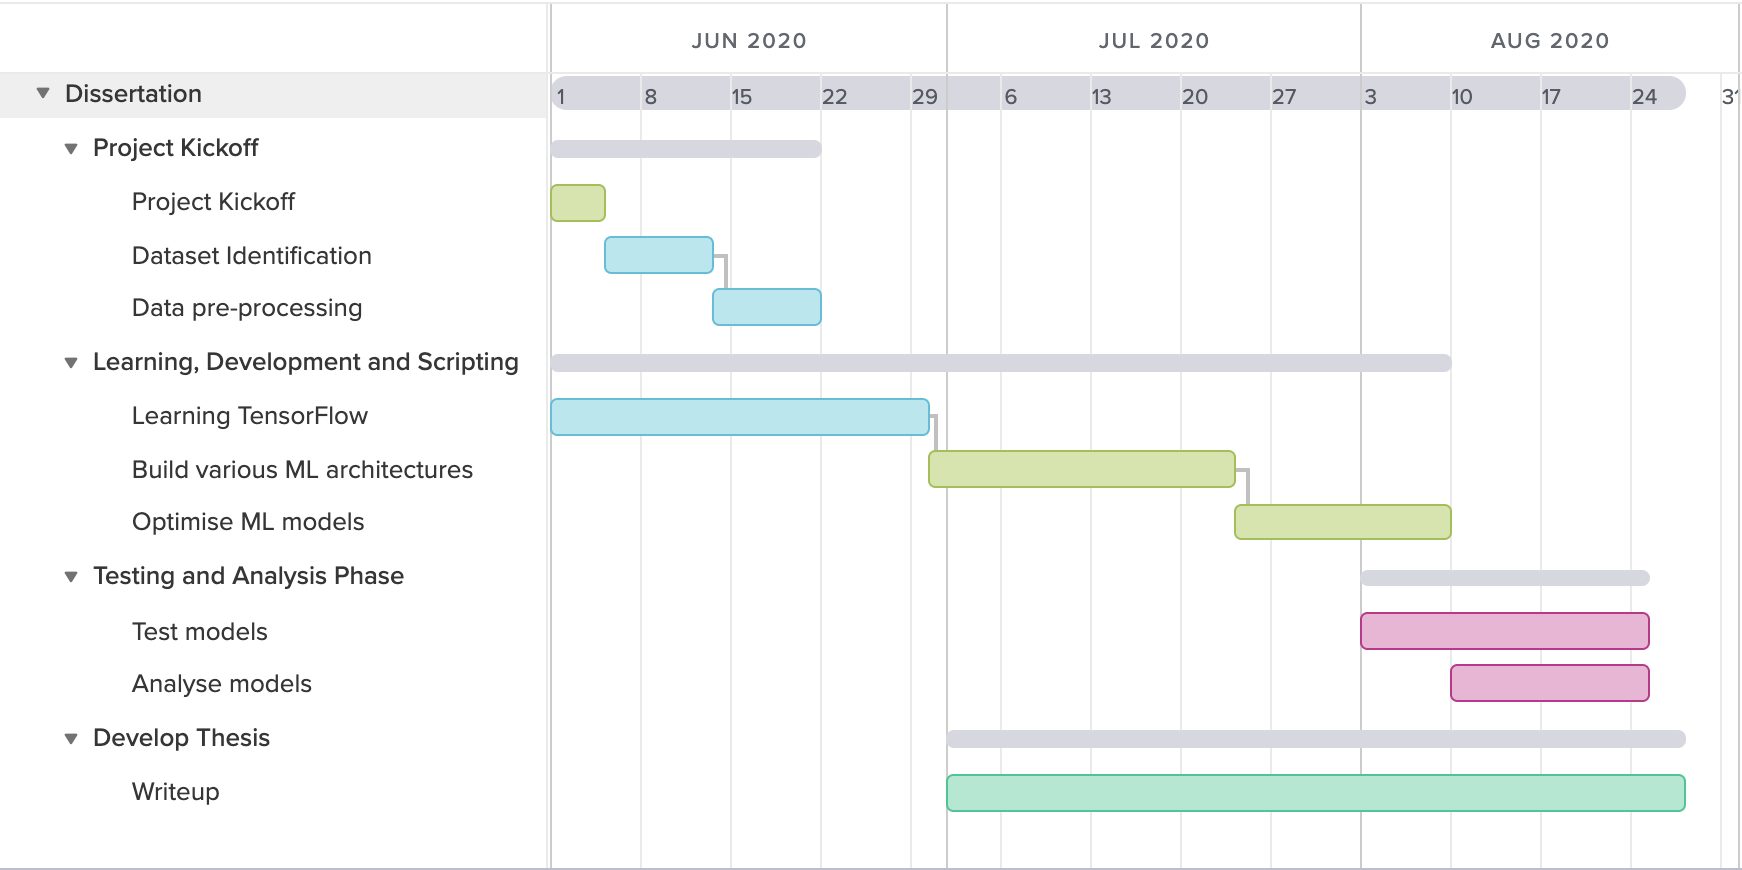
\includegraphics[width=\linewidth,scale=0.5]{timeline.png}
  \caption{dsadsadsa}
\end{figure}
   
\printbibliography
 
\end{document}